% Chap 1. Introduction
\chapter{緒論}
\label{c:intro}
\section{這是1-1章}
這邊是1-1節!根據\cite{Rowe:2005:ASR}的說法,這邊就是這個那個這個那個

\newpage
\section{這是1-2章}
這邊是1-2節!試著放個圖:
\begin{figure}[h!]
\centering
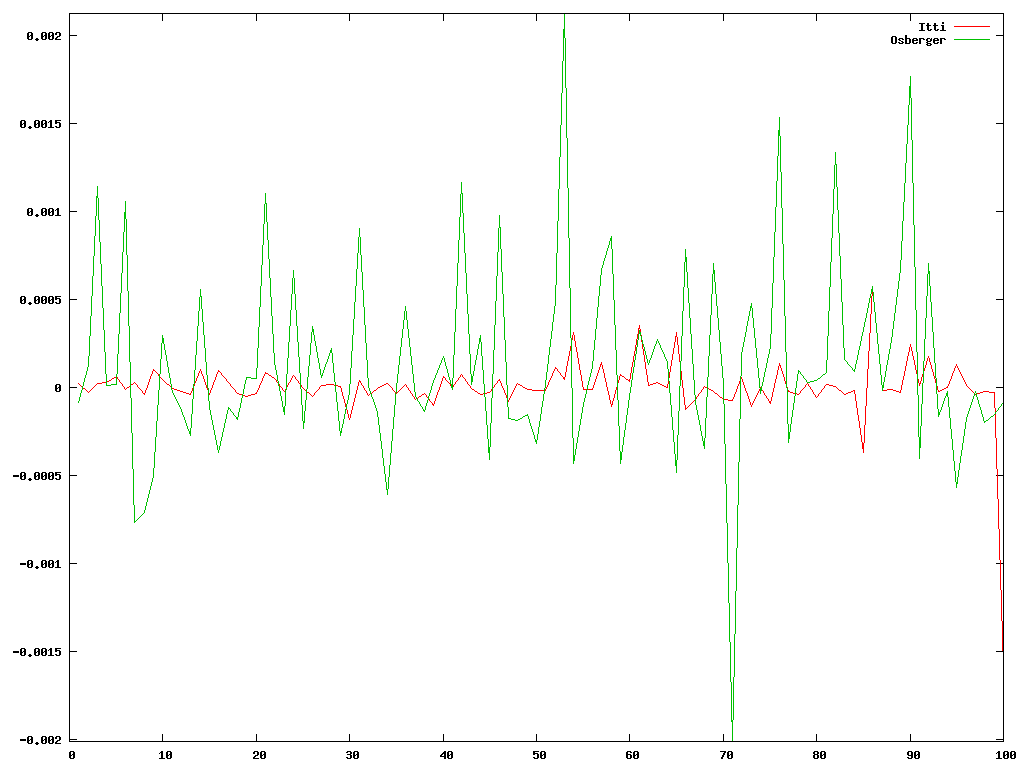
\includegraphics[width=0.45\textwidth]{sample}
\caption{這是範例圖}
\label{kl}
\end{figure}

再試著放個表:
\begin{table}[h!]
\begin{center}
\begin{tabular}{lcc}

\hline
                    &  {\small Itti's method}     & {\small Fuzzy growing}    \\
\hline
{\small Precision}           &  0.4475    & 0.4506 \\
{\small Recall}              &  0.5515    & 0.5542 \\
\hline

\end{tabular}
\caption{這是範例表}
\label{t:FOA}
\end{center}
\end{table}

就這樣啦!
